\section{\uppercase{Photograph-Preserving Extension}}
\label{sec:cover-supp}
This allocation adds 52 carriers, twelve development and forty held-out, not repetitions of the generated-PNG study. Training identifiers are 2092, 8049, 8143, 12003, 12074 and 15004. Test identifiers are 2018, 3063, 5096, 6046, 8068, 10081, 14085, 14092, 15011, 15062, 16004, 16068, 17067, 20069, 23050, 28083, 29030, 33044, 35028 and 35049. These are the lowest numeric filenames in the respective partitions, fixed before embedding. All canonical covers are RGB center crops with floor offsets and no resize, from the January 2013 BSDS500 distribution \cite{bsds}. Text assignments retain the original six development and twenty held-out byte sequences and provenance. There are twenty independent evaluation cover/text groups, not forty independent paired comparisons.\aifootnote

\begin{figure*}[t]
\centering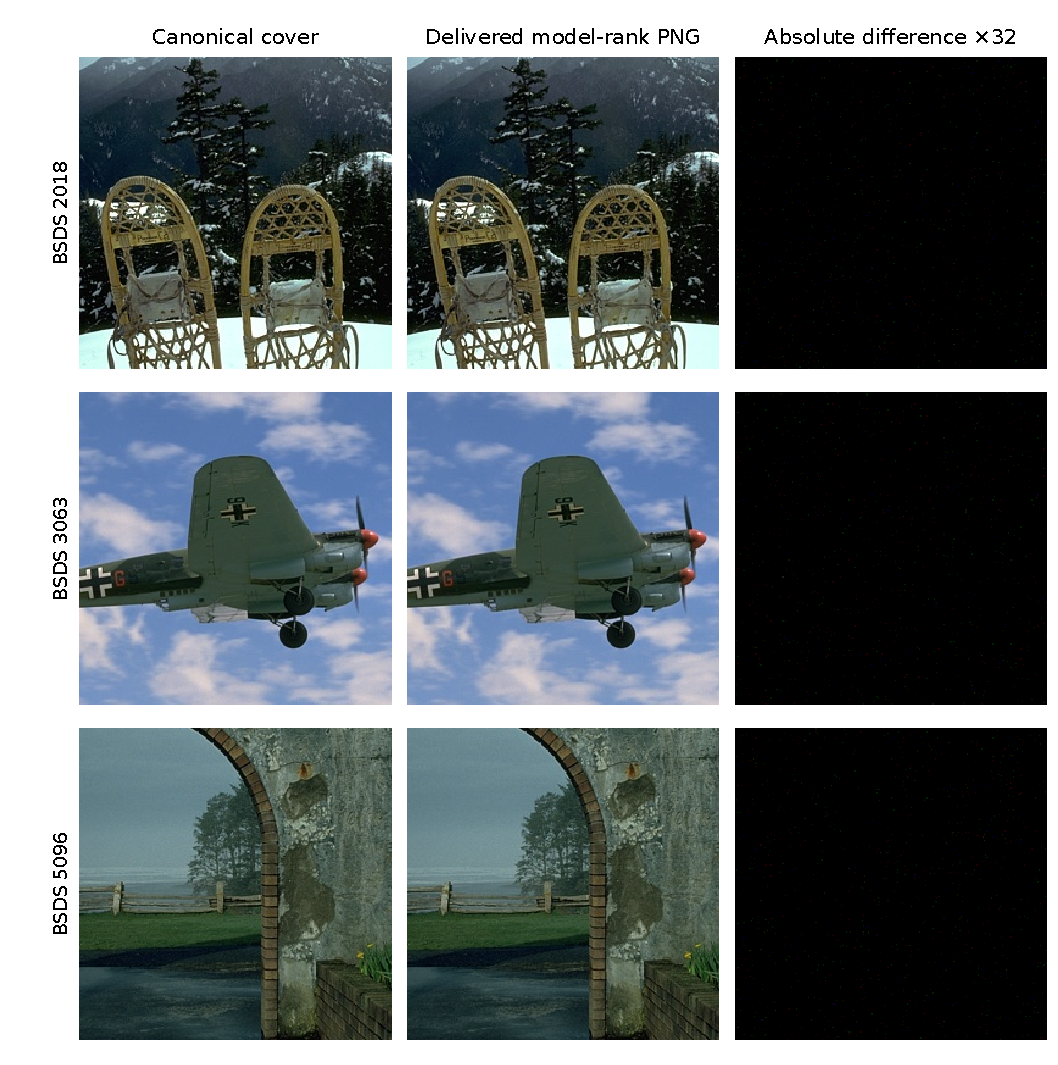
\includegraphics[width=\textwidth]{figures/cover_examples.pdf}
\caption{The first three frozen held-out photographs in the model-rank arm. Columns show canonical cover, actual delivered PNG and absolute channel difference amplified by 32, respectively. Black denotes no change. The sparse differences are intentionally faint at this fixed amplification. Both images are $256\times256$ RGB8, displayed with nearest-neighbor enlargement and no enhancement. Distortion is measured against the canonical crop, not the original JPEG container. Selection was by identifier, not visual appeal or recovery outcome. These images illustrate preservation, not human-observer or steganalysis results.}
\label{fig:cover-differences}
\end{figure*}

\subsection{Deterministic Placement and Candidate Scoring}
The domain-separated placement key is HKDF-SHA256 of the 32-byte run key, with salt SHA256 of row-major coarse RGB bytes. Its info is the ASCII prefix \texttt{ImageCalgacus/cover\_rank\_v1/placement}, one zero byte and the 32-byte canonical protocol hash. Canonical JSON uses sorted keys, compact separators and UTF-8. This protocol identity includes the pinned checkpoint and all rank-map rules, but excludes arm and local runtime paths. For each raster index $i$, compute HMAC-SHA256 of \texttt{pixel}, one zero byte and unsigned four-byte big-endian $i$. Sort digests lexicographically, breaking collisions by $i$. The first 2,336 indices give bit order. No hidden nonce or sender end position is required.

The original packet remains nonce, ciphertext and tag, totaling 292 bytes. Each cover/text group is encrypted once using a fresh run key and a distinct random nonce. Both arms transport that immutable packet. Each pixel's lexicographic cube spans its three four-value coarse cells. Rank parity partitions all 64 candidates into classes of 32. The sender's nearest-candidate decision uses original RGB values, but only the observed rank class is needed to decode. Only the selected pixels may change.

The joint log-mass calculation uses the common mixture weights and candidate-specific red/green conditioning. It does not multiply independent channel marginals, discard underflowed candidates or use the training loss's small-density approximation. A predetermined three-tile development probe matches reference and CUDA graph parameter maps exactly. Joint log scores agree with the existing sequential conditional implementation to at most $1.07\times10^{-14}$ log units. All 26 model-arm senders and fresh receivers reproduce exact map, score and ordering digests. This tolerance concerns the independent formula check, not acceptance of nonidentical sender/receiver ranks.

For label vectors $L$ and $C$, partition disagreement is
\begin{equation}
d(L,C)=\min\{h(L,C),64-h(L,C)\}/64,
\end{equation}
where $h$ is Hamming distance over the same ordered candidate cube. Allowing the complement avoids mistaking a global bit-label swap for a new partition. Every selected development and held-out partition differs from parity. The held-out per-image mean ranges from 0.44658 to 0.45116, averaging 0.44844.

\subsection{Fidelity, Failure Checks and Runtime}
The model arm's held-out PSNR ranges from 70.091 to 70.494 dB. Its SSIM ranges from 0.9999404 to 0.9999874. Parity PSNR ranges from 70.308 to 70.610 dB. Channel changes are at most two for model ranks and one for parity. Mean changed-channel fractions are 0.6133\% and 0.5933\%, respectively. Mean PNG file sizes are 116,772.85 and 116,762.50 bytes. Both carry a mean 93.2 useful bytes in the same 2,336-bit packet. The model-minus-parity paired mean SSIM difference is $-2.388\times10^{-6}$ and file-size difference is 10.35 bytes. These are descriptive summaries, not evidence of statistical or security superiority.

The independent worst-case bound uses total squared error at most $2336\times3\times9=63,072$, giving $\mathrm{PSNR}\geq53.06845$ dB. It is conservative because not all selected pixels change and nearest candidates usually differ in one channel. PSNR uses peak 255 and all RGB samples. SSIM uses valid centers of an $11\times11$ Gaussian window with standard deviation 1.5, population covariance, data range 255, $K_1=.01$ and $K_2=.03$, then averages channels. A constant-image fixture checks the metric against its closed-form value.

Six verification receivers operate on the first development cover, one wrong key, one changed embedded bit and one lossless re-save per arm. Four expected authentication rejections produce no plaintext. Both compression-9 re-saves preserve exact pixels and recover. They are checks, not additional independent carriers. No unexpected protocol or infrastructure failure occurs. An unused low-bit mutation can leave the message intact, so GCM is not whole-image authentication.

All 56 neural jobs verify CUDA allocation, parameter/input placement, strict loading, inference mode and positive process-specific activity. Each complete image uses 64 graph forwards in addition to setup. The model arm's mean held-out encoding phase is 2.122 seconds and decoding phase 1.983 seconds. Cold model loading averages 0.973 and 0.982 seconds. These intervals are nested within charged process totals, not additional costs. The entire extension charges 429.149 seconds, including 387.756 seconds for neural processes and a conservatively charged 41.393 seconds for 55 model-free child processes. Cumulative project accounting becomes 89,404.217 seconds, below 144,000. Neither the remaining allocation nor this result authorizes further experiments.

\subsection{Scope and Reproduction}
The trained model was not optimized for this cover distribution. Reconstructible partitions are demonstrated, but their measured fidelity and runtime do not improve upon simple parity. Neither visual inspection nor PSNR/SSIM establishes undetectability. No trained steganalyzer, human study, JPEG transform or learned-watermark robustness comparison was run.

Public verification recomputes image metrics, checks source equality, hashes, allocation and recorded GPU evidence without keys or neural execution. Fresh reproduction additionally requires the pinned checkpoint, compatible CUDA runtime, retained run key and the agreed profile. The receiver receives only carrier, profile/arm and key. Public source-containing evidence directories are not receiver inboxes. Original packets, wrong-key files and detailed private traces are excluded from manuscript assets. Dataset citation is provided, but blanket photograph republication permission was not identified in the mirror; publication reuse remains an author check.
